\documentclass[fleqn,answers,addpoints]{exam}

%\usepackage{graphicx, fancyhdr}
\usepackage{etoolbox}
\usepackage{subcaption}
\usepackage{etoolbox}
\usepackage{tikz,pgfplots}
\usepackage{amsmath, amsfonts}
\usepackage{color}

%% For LaTeX-Box: root = stat105_exam1_info.tex 
%%%%%%%%%%%%%%%%%%%%%%%%%%%%%%%%%%%%%%%%%%%%%%%%%%%%%%%%%%%%%%%%%%%%%%%%%%%%%%%%
%  File Name: stat105_exam1_info.tex
%  Purpose:
%
%  Creation Date: 24-09-2015
%  Last Modified: Thu Sep 24 13:51:36 2015
%  Created By:
%%%%%%%%%%%%%%%%%%%%%%%%%%%%%%%%%%%%%%%%%%%%%%%%%%%%%%%%%%%%%%%%%%%%%%%%%%%%%%%%
\newcommand{\course}[1]{\ifstrempty{#1}{STAT 105}{STAT 105, Section #1}}
\newcommand{\sectionNumber}{B}
\newcommand{\examDate}{October 1, 2015}
\newcommand{\semester}{FALL 2015}
\newcommand{\examNumber}{II}

\newcommand{\examTitle}{Exam \examNumber}

\runningheader{\course{\sectionNumber}}{Exam \examNumber}{\examDate}
\runningfooter{}{}{Page \thepage of \numpages}

\newcommand{\examCoverPage}{
   \begin{coverpages}
   \centering
   {\bfseries\scshape\Huge Exam I \par}
   \vspace{1cm}
   {\bfseries\scshape\LARGE \course{\sectionNumber} \par}
   {\bfseries\scshape\LARGE \semester \par}

   \vspace{2cm}

   \fbox{\fbox{\parbox{5.5in}{\centering 

      \vspace{.25cm} 
      
      {\bfseries\Large Instructions} \\

      \vspace{.5cm} 

      \begin{itemize}
         \item  The exam is scheduled for 80 minutes, from 8:00 to 9:20 AM. At 9:20 AM the exam will end.\\
         \item  A forumula sheet is attached to the end of the exam. Feel free to tear it off.\\
         \item  You may use a calculator during this exam.\\
         \item  Answer the questions in the space provided. If you run out of room, continue on the back of the page. \\
         \item  If you have any questions about, or need clarification on the meaning of an item on this exam, please ask your instructor. No other form of external help is permitted attempting to receive help or provide help to others will be considered cheating.\\
         \item  {\bfseries Do not cheat on this exam.} Academic integrity demands an honest and fair testing environment. Cheating will not be tolerated and will result in an immediate score of 0 on the exam and an incident report will be submitted to the dean's office.\\
      \end{itemize}

   }}}

   \vspace{2cm}

   \makebox[0.6\textwidth]{Name:\enspace\hrulefill}

   \vspace{1cm}

   \makebox[0.6\textwidth]{Student ID:\enspace\hrulefill}
   \end{coverpages}

}


\newcommand{\course}[1]{\ifstrempty{#1}{STAT 305}{STAT 305, Section #1}}
\newcommand{\sectionNumber}{3}
\newcommand{\examDate}{December 18, 2019}
\newcommand{\semester}{Fall 2019}
\newcommand{\examNumber}{}
\newcommand{\qparts}[1]{\begin{parts} #1 \end{parts}}
\newcommand{\qitems}[1]{\begin{itemize} #1 \end{itemize}}

% Document definitions
\newcommand{\examTitle}{\examNumber Final Exam }
\runningheader{\course{\sectionNumber}}{\examNumber Final Exam }{\examDate}
\runningfooter{}{}{Page\ \thepage\ of\ \numpages}

\begin{document}
	
	\begin{coverpages}
		\centering
		{\bfseries\scshape\Huge \examNumber Final Exam  \par}
		\vspace{1cm}
		{\bfseries\scshape\LARGE \course{\sectionNumber} \par}
		{\bfseries\scshape\LARGE \semester \par}
		\vspace{2cm}
		\fbox{\fbox{\parbox{5.5in}{
					\centering 
					\vspace{.25cm} 
					{\bfseries\Large Instructions} \\
					\vspace{.25cm} 
					\begin{itemize}
						\item  The exam is scheduled for 120 minutes, from 09:45 AM to 11:45 AM. At  11:45 AM  the exam will end.\\
						\item  Total points for the exam is 100. Points for individual questions are given at the beginning of each problem. Show all your calculations clearly to get full credit. Put final answers in the box at the right (except for the diagrams!).
						\item  A formula sheet is attached to the end of the exam. Feel free to tear it off.\\
						\item  You may use a calculator during this exam.\\
						\item  Answer the questions in the space provided. If you run out of room, continue on the back of the page. \\
						\item  If you have any questions about, or need clarification on the meaning of an item on this exam, please ask your instructor. No other form of external help is permitted attempting to receive help or provide help to others will be considered cheating.\\
						\item  {\bfseries Do not cheat on this exam.} Academic integrity demands an honest and fair testing environment. Cheating will not be tolerated and will result in an immediate score of 0 on the exam and an incident report will be submitted to the office of the dean.\\
					\end{itemize}
		}}}
		\vspace{1cm}
		\makebox[0.6\textwidth]{}
		\vspace{1cm}
		\makebox[0.6\textwidth]{Name:\enspace\hrulefill}
		\vspace{1cm}
		\makebox[0.6\textwidth]{Student ID:\enspace\hrulefill}
	\end{coverpages}
	
	\begin{questions}
		
		\question[2]A random sample of 1000 students' Statistics exam scores was
drawn from the population of all possible comparable Stat exam scores
(an unknown population/distribution). The sample mean, once computed,
has the exact value of the distribution/population mean.

\begin{oneparchoices}
\choice True
\choice False
\end{oneparchoices}
\vspace{0.5cm}

\question[2]While trying to figure out the probability that the sample
mean for a data of size 10 would exceed a value, we can apply the
central limit theorem.

\begin{oneparchoices}
\choice True
\choice False
\end{oneparchoices}
\vspace{0.5cm}

\question

An agriculturist is attempting to determine which of three species of
corn (A, B, and C) yield the most grain per acre. Since the yield may
depend on the fertilizer used, the researcher intends to use fertilizers
with different concentrations of Nitrogen as well - low Nitrogen,
medium-low Nitrogen, medium-high Nitrogen, and high Nitrogen. There are
8 fields (scattered around Iowa) available to perform this expiriment.
Each field is divided into 24 single acre plots and the combinations of
species and fertilizer are randomly assigned so that within each field
every combination is used exactly twice. Since the size of the plants
may impact their growth when placed close by each other, it was decided
that all species would be planted in a grid with each plant exactly four
feet from its nearest neighbor. The agriculturalist also decided not to
use any pest control system during growth. At harvest time, the weight
of grain each plot yields is recorded and the combination of corn
species and fertilizer that gives the highest average yield is chosen.

\qparts{
\part[2] Explain why this is an experiment and not an observational study. \vspace{2cm}
\part Identify each of the following and describe them as numeric (in which case, identify whether it is continuous or discrete) or categorcial (in which case list the possible levels). \vspace{1cm}
\begin{subparts}
   \subpart[2] Identify the response variable(s): \vspace{2cm}
   \subpart[2] Identify the experimental variable(s): \vspace{2cm}
   \subpart[2] Blocking variable(s): \vspace{2cm}
\end{subparts}
\part[2] Identify two controlled variables used in this process. \vspace{2cm}
}

\newpage
\question

A survey given to members of a national engineering society who
graduated five years prior is attempting to determine the relationship
between salary and undergraduate GPA. The graph below displays 150
responses.

\begin{center}

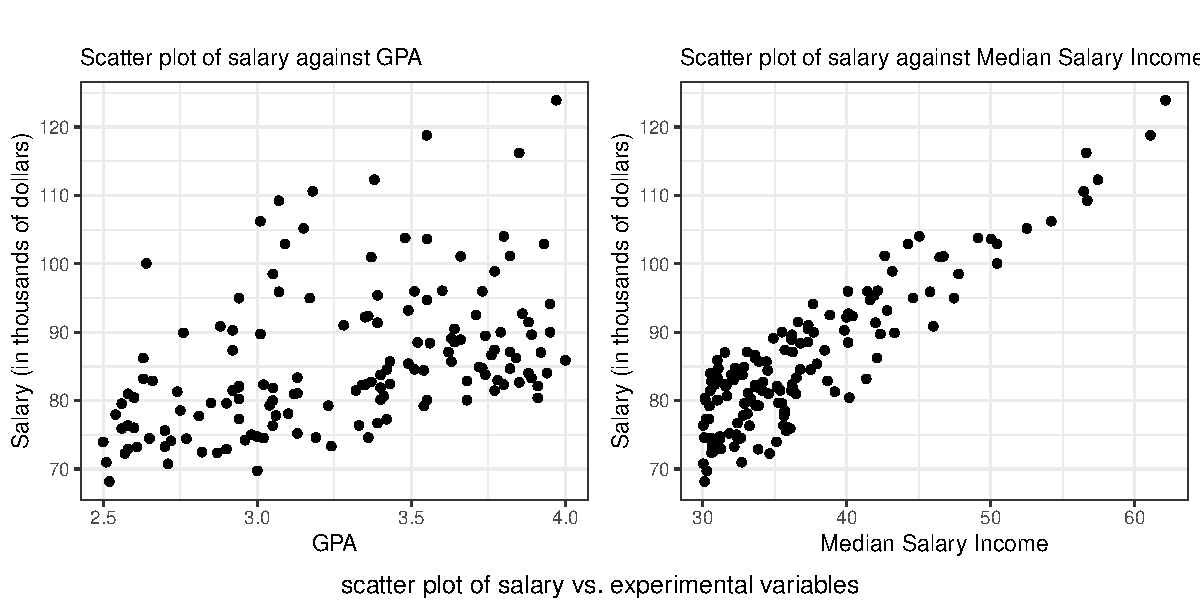
\includegraphics[width=.9\linewidth]{stat305_final_F19_files/figure-latex/unnamed-chunk-3-1} 
\end{center}

The normal qq-plot of residual of the fit and the residual vs.~predicted
plot are as follows:

\vspace{0.5cm}
\centerline{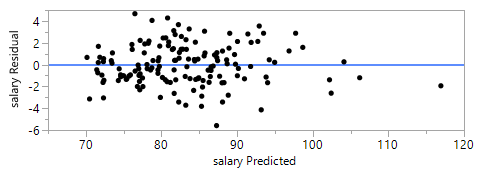
\includegraphics[scale=0.8]{salary_res}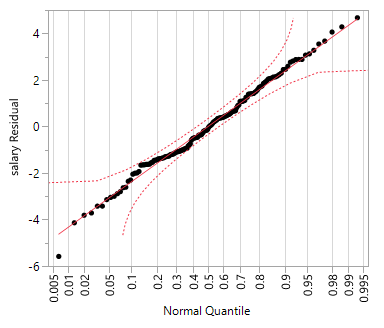
\includegraphics[scale=0.8]{salary_q}}
\captionof{figure}{Residual vs. predicted variables (the left) and Normal quantile plot (the right)}

\vspace{0.5cm}

\qparts{
\part[2] Looking at the two plots above, are the assumptions of the regression model met?
}
\newpage

Discouraged by the relationship between salary and GPA, the surveyors
remember that they know the address of each respondant and are able to
determine the median income of the area in which the respondant lives.

The JMP output below comes from fitting a linear relationship using for
annual salary of the respondant (``\verb!salary!'') using both the
undergraduate GPA (``\verb!GPA!'') and the median income of the area in
which the respondant lives (``\verb!med_salary_loc!'') (in thousands of
dollars).

\vspace{1cm}
\centerline{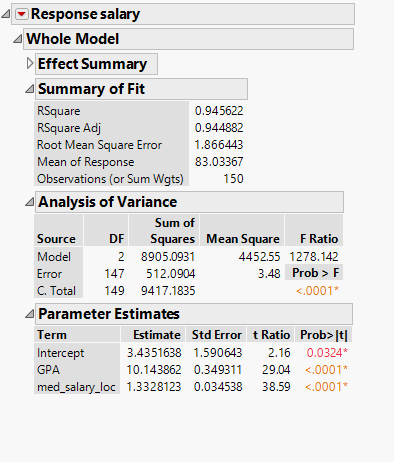
\includegraphics[scale=1]{salary_fit}}
\vspace{1cm}

\qparts{
\part[3] Using the JMP output, write the equation of the fitted multivariate linear relationship between GPA, median salary income  and salary 

\hfill \fbox{ \textcolor[rgb]{1.00,1.00,1.00}{$\bigcap$} \hskip -0.4cm $\hat y =$ \hspace{10cm}}
\vspace{3cm}
\newpage
\part[3] Using this fitted multivariate linear relationship, what do we suppose the salary would be for an engineer with a undergraduate GPA of 2.63 living in a location with a median income of 32.43 thousand dollars?

\hfill \fbox{ \textcolor[rgb]{1.00,1.00,1.00}{$\bigcap$} \hskip -0.4cm $\hat y =$ \hspace{10cm}}
\vspace{3cm}
\part[3] The actual salary of one engineer surveyed with a undergraduate GPA of 2.63 living in a location with a median income of \$32,430 was \$74,340.  What is the residual for this specific engineer's actual salary using the fitted multivariate linear relationship? 
\hfill \fbox{ \textcolor[rgb]{1.00,1.00,1.00}{$\bigcap$} \hskip -0.4cm $\text e =$ \hspace{2cm}}
\vspace{4cm}
\part[4] For the linear relationship, find \(r\), the sample correlation coeffecient and \(R^2\), the coeffecient of determination.
\hfill \fbox{ \textcolor[rgb]{1.00,1.00,1.00}{$\bigcap$} \hskip -0.4cm $r=$ \hspace{2cm}}

\hfill \fbox{ \textcolor[rgb]{1.00,1.00,1.00}{$\bigcap$} \hskip -0.4cm $R^2=$ \hspace{2cm}}


\vspace{3cm}
\part[3] For your response for \(R^2\) in previous part, provide an interpretation.\vspace{3cm}
\part[3] Provide an estimate for $\sigma^2$. 
\hfill \fbox{ \textcolor[rgb]{1.00,1.00,1.00}{$\bigcap$} \hskip -0.4cm $\hat\sigma^2 = s_{SF}^2=$ \hspace{2cm}}
\vspace{2cm}
\newpage
\part[3] Provide an estimate for the \emph{variance} of the coefficient of \emph{GPA}. 
\hfill \fbox{ \textcolor[rgb]{1.00,1.00,1.00}{$\bigcap$} \hskip -0.4cm $\text{Var}(b_1) =$ \hspace{2cm}}
\vspace{3cm}
\part[5] Calculate and intepret the $95\%$ two-sided confidence interval for the coefficient of \emph{GPA}. 
\hfill \fbox{ \textcolor[rgb]{1.00,1.00,1.00}{$\bigcap$} \hskip -0.4cm $(\hspace{3cm},\hspace{3cm} )$ }
\vspace{6cm}

\part[10] Conduct a formal hypothesis test at the $\alpha = 0.05$ significance level to determine if there is significance relationship between salary (y) and  \emph{median salary income} $(x_1)$, holding GPA constant. \\
\emph{Note: Write down all six steps for full credit.}
}

\newpage
\text{You may use this blank space for completing the steps of hypothesis test}\vspace{8cm}

\question

A team of engineers is studying the differences in camera systems on
self-driving cars. Their primary concern is in the car's ability to
avoid obstacles. Each system was installed in a test car and on 10
consecutive days the car was sent on a 15 hour drive through a closed
obstacle course where the number, timing, location, and type of obstacle
the car encounters is randomly determined. The proportion of obstacles
avoided during the 15 hour drive is independently recorded below (along
with relevant summary statistics):

\begin{itemize}
\item System 1: 0.82, 0.83, 0.82, 0.79, 0.8, 0.83, 0.77, 0.84, 0.8, 0.86 (with $\bar{x_1} = 0.82, s_1^2 = 0.0007$)
\item System 2: 0.77, 0.79, 0.75, 0.73, 0.75, 0.75, 0.82, 0.78, 0.8, 0.76 (with $\bar{x_2} = 0.77, s_2^2 = 0.0008$)
\end{itemize}

\emph{Note: there are 10 sample data of each system. i.e $n_1= n_2= 10$}
\vspace{.3cm} \qparts{
\part[5] Provide a 95\% confidence interval for the mean proportion of obstacles avoided on the course using System 1.
\hfill \fbox{ \textcolor[rgb]{1.00,1.00,1.00}{$\bigcap$} \hskip -0.4cm $(\hspace{3cm},\hspace{3cm} )$ }
\vspace{4cm}
\part[5] Provide a one-sided 95\% lower bound confidence interval for the mean proportion of obstacles avoided on the course using System 2. 
\hfill \fbox{ \textcolor[rgb]{1.00,1.00,1.00}{$\bigcap$} \hskip -0.4cm $(\hspace{3cm},\hspace{3cm} )$ }
\vspace{3cm}
\newpage
\part[10] Assuming that the proportion of obstacles avoided is roughly normally distributed and that the both systems have the same variance in proportion of obstacles avoided, conduct a hypothesis test at the $\alpha = 0.05$ significance level for the claim that the true mean of the obstackes avoided of the two systems are significantly different.\\
\emph{Note: Write down all six steps for full credit.}
 \vspace{4cm} 
}

\newpage
\question

Let \(X\) be a normal random variable with a mean of -2 and a varaince
of 16 (i.e., \(X \sim N(-2, 16)\)) and let \(Z\) be a random variable
following a standard normal distribution. Find the following
probabilities (note: the attached standard normal probability table may
be helpful):

\qparts{
\part[2] $P(Z \le 1.0)$ \vspace{3cm}
\part[2] $P(|Z| \le 2.5)$ \vspace{3cm}
\part[2] $P(-8 \le X < 1)$ \vspace{4cm}
\part[3] $P(|X| \ge 4)$ \vspace{4cm}
\part[5] find c such that $P(|X| \le c)= 0.95$\vspace{8cm}
}

\question Seventy independent messages are sent from an electronic
transmission center. Messages are processed sequentially, one after
another. Transmission time of each message is Exponential with parameter
\(\alpha = 10\)min.\\
\qparts{
\part[3] what are the expected value and variance of the sample mean of all 70 messages? 

\hfill \fbox{ \textcolor[rgb]{1.00,1.00,1.00}{$\bigcap$} \hskip-0.4cm $\text{E}(\overline{X}) =$ \hspace{2.35cm}}

\hfill \fbox{ \textcolor[rgb]{1.00,1.00,1.00}{$\bigcap$} \hskip-0.4cm $\text{Var}(\overline{X}) =$ \hspace{2cm}}
\vspace{4cm}

\part[4] Find the probability that the average of all 70 messages are transmitted in less than 8 minutes. 
\hfill \fbox{ \textcolor[rgb]{1.00,1.00,1.00}{$\bigcap$} \hskip-0.4cm $\text{p} =$ \hspace{2cm}}
\vspace{4cm}
}

\newpage

\question

Two independent discrete random variab1e \(X\) and \(Y\) can be
described using the following probability functions:

\begin{table}[ht]
\begin{minipage}[b]{0.5\linewidth}\centering
\begin{tabular}{c|cccc}
%\hline
$x$ &$-1$& 0&1&2\\
\hline
$f_X(x)$ & 0.2&0.3 & 0.3&0.2\\
%\hline
\end{tabular}
\end{minipage}
\hspace{0.5cm}
\begin{minipage}[b]{0.5\linewidth}
\centering
\begin{tabular}{c|cccc}
%\hline
$y$ &1& 2&3&4\\
\hline
$f_Y(y)$ & 0.3&0.2 & 0.2&0.3\\
%\hline
\end{tabular}
\end{minipage}
\end{table}

\%

\qparts{
\part[4] Find the means and standard deviations for $X$ and $Y$
respectively.

\vskip 8cm

 \hfill
\fbox{ \textcolor[rgb]{1.00,1.00,1.00}{$\bigcap$} \hskip -0.4cm
$\mu_X$ = \hspace{2cm} $\sigma_X=$\hspace{2cm}}

 \hfill
\fbox{ \textcolor[rgb]{1.00,1.00,1.00}{$\bigcap$} \hskip -0.4cm
$\mu_Y$ = \hspace{2cm} $\sigma_Y=$\hspace{2cm}}

\part[2] Find  the mean and standard deviation
for the random variable $2X - 3Y + 5$.

\vskip 3cm

 \hfill
\fbox{ \textcolor[rgb]{1.00,1.00,1.00}{$\bigcap$} \hskip -0.4cm mean
= \hspace{2cm} s.d=\hspace{2cm}}
}
		
	\end{questions}
	
\end{document}
